\documentclass[11pt]{article}

\usepackage[margin=1in, paperwidth=8.5in, paperheight=11in]{geometry}
\usepackage{amsmath}
\usepackage[document]{ragged2e}
\usepackage{graphicx}
\usepackage{listings}
\usepackage{color}
\usepackage{interval}
\usepackage[none]{hyphenat}

\definecolor{dkgreen}{rgb}{0,0.6,0}
\definecolor{gray}{rgb}{0.5,0.5,0.5}
\definecolor{mauve}{rgb}{0.58,0,0.82}


\lstset{
  frame=tb,
  language=Python,
  aboveskip=3mm,
  belowskip=3mm,
  showstringspaces=false,
  columns=flexible,
  basicstyle={\small\ttfamily},
  numbers=none,
  numberstyle=\tiny\color{gray},
  keywordstyle=\color{blue},
  commentstyle=\color{dkgreen},
  stringstyle=\color{mauve},
  breaklines=true,
  breakatwhitespace=true,
  tabsize=3,
  breaklines=true 
}


\begin{document}

\title{\textbf{Homework 3}}
\author{Dejan Porjazovski}
\maketitle

\section{Problem 1 : clustering given a hierarchy}
\subsection{Show that the problem of k-means on trees can be solved optimally in polynomial time}
Below is a pseudo code of the algorithm \\

\begin{lstlisting}
# We use a bottom-up approach and do tree traversal from the bottom

recursion to get to the bottom of the tree
then
if element has children:
	element_left_index = indexOf(element.left)
	element_right_index = indexOf(element.right)
	# get the arrays of those elements 
	element_left = complete_array[element_left_index]
	element_right = complete_array[element_right_index]
	left_right = element_left + element_right
	sum_left_right = sum(element_left.elements + element_right.elements)
	n = len(element_left.elements) + len(element_right.elements)
	variance = sum_left_right^2 - sum_left_right/n
	self_element = [1, variance, [node_index], [element_left.elements, element_right.elements]]	
	
	complete_array.append([left_right, self_element])


else:
	# if it's 1 element, then it has 0 variance
	complete_array.append([1, 0, [node_index], [value]])

at the end
find elements with same amount of clusters
remove the element that has higher variance
return complete_array
\end{lstlisting}

The algorithm might not be that clear so I will try to explain it with words and an example.
\newpage
First thing to note is that we use a bottom-up approach and use tree traversal algorithm (for example postorder) to visit the nodes of the tree. \\
First we get to the leaf nodes. The leaf nodes have 0 variance and can be treated as clusters on their own. \\
We store an array for each node that we visit. The array contains the number of elements in that node, the variance, the indices of the elements the node contains and the values of those elements. \\
For example for a leaf node we can have $ [1, 0, [v4], [3]] $ where v1 is the index of the element itself because the leaf nodes contain only one element. \\
If we visit a node that has children, then we put in the array the sum of the elements of the left and right child and we also store the element itself. \\ 
The element itself has variance calculated for all its children. \\
We repeat the approach unltil we get to the top of the tree. \\
At the end we find the elements in the array that have same amount of clusters and discard the element with higher variance. \\~\\
Below is a concrete example of the algorithm.

\begin{center}
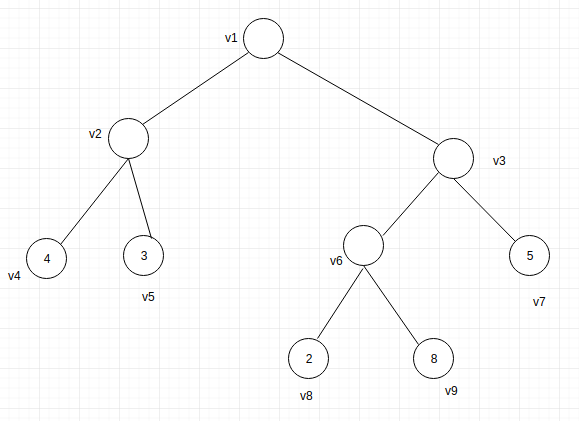
\includegraphics[width=18cm, height=7cm]{tree.png}
\end{center}
Consider we have the tree shown above. \\
We traverse to the leafs of the tree. Lets say we start from the v4 node. \\
For each node we keep an array of 4 values: number of elements in the node, the variance of the elements in the node, the node indices and the elements the node has. \\
For the v4 node we get: \\
$ i_4 [ 1,0,[v_4], [4]] $ \\
Then we move to the next node, v5: \\ 
$ i_5 [1,0,[v_5], [3]] $ \\
Now we move the the node v2, where we calculate $ i_{2_{self}} $, which is the node itself with the variance of it's children nodes. We also calculate the sum of the left and right children of that node:
$$ i2 = [(i4 + i5), i2_{self}] $$
which looks like this: \\
$ [2, 0, [v4, v5], [4,3]] $ which is left + right child \\
then we calculate the variance with the equation: $ \sum(x_i^2) - \frac{\sum(x_i)^2}{N} $ and then calculate $ i2_{self} $: \\
$ [1, 0.5, [v2], [4,3]] $, so, at the end, the t2 array looks like this: \\
$ i2 = [ [1, 0.5, [v2], [4,3]], \: [2, 0, [v4, v5], [4, 3]] ] $ \\~\\
Then we move to the next node, which is v8. \\
For v8 we have $ [1, 0, [v8], [2]] $. \\
For v9 we have $ [1, 0, [v9], [8]] $. \\
Now we move to the v6 node and we do the same thing as we did with the v2 node: \\
We need to calculate $ i6 = [(i8 + i9), i6_{self}] $ \\
First we sum left and right nodes (v8 and v9): \\
$ 2, 0, [V8, V9], [2, 8] $ \\
For $ i6_{self} $ we have $ [1, 18, [v6], [2, 8]] $. \\~\\
We repeat this process until we get to the root of the tree. \\
We get an array that looks like this: \\

$ [ $ \\
$ [1, 21, [v1], [4, 3, 2, 8]] $ \\
$ [2, 7.7, [v2, v3], [4, 3, 2, 8]] $ \\
$ [3, 18.5, [v2, v6, v7], [4, 3, 2, 8]] $ \\
$ [4, 0.5, [v2, v7, v8, v9], [4, 3, 2, 8]] $ \\
$ [3, 7.2, [v3, v4, v5], [4, 3, 2, 8]] $ \\
$ [4, 18, [v4, v5, v6, v7], [4, 3, 2, 8]] $ \\
$ [5, 0 , [v4, v5, v7, v8, v9], [4, 3, 2, 8]] $ \\
$ ] $ \\~\\
From here we can see that we have two option for forming 3 and 4 clusters so, we choose the ones with the smallest variance and remove the others. \\
The final array look like this: \\
$ [ $ \\
$ [1, 21, [v1], [4, 3, 2, 8]] $ \\
$ [2, 7.7, [v2, v3], [4, 3, 2, 8]] $ \\
$ [4, 0.5, [v2, v7, v8, v9], [4, 3, 2, 8]] $ \\
$ [3, 7.2, [v3, v4, v5], [4, 3, 2, 8]] $ \\
$ [5, 0 , [v4, v5, v7, v8, v9], [4, 3, 2, 8]] $ \\
$ ] $ \\~\\

Now, for example if we have $ k=3 $, then we choose $ [3, 7.2, [v3, v4, v5], [4, 3, 2, 8]] $, which mean that the most optimal 3 clusters are the nodes $ v3, v4, v5 $.

\subsection{Show the correctness of your algorithm}
At the end of the algorithm we get all the clusters that can appear in the tree and their variances. If there are multiple ways of forming k-clusters, then we choose the combination that has the lowest variance so, the algorithm always produces the most optimal k-clusters.

\subsection{What is the complexity of your algorithm?}
The postorder tree traversal has complexity of $ O(n) $. We need to calculate approximately $2n - 1 = n$ arrays to get to the top of tree and have the clusters. The variance calculation takes $ O(4n) $. The complexity of calculating an array is $ 4n * n  = 4n^2 = n^2 $. The complexity of the algorithm is: \\
$ n^2 * n = n^3 $, which is polynomial time.



\section{Clustering a data stream}

\subsection{Prove that the STREAMING - FURTHEST algorithm produces a clustering that has at most k cluster centers}
We will try to prove this by contradiction. \\
Let's consider a case where we get k+1 centers: $ l>k $. \\
We know the optimal k-centers cost $d^*$.
We also know that the distance from the new element to it's closes center should be $ \leq 2d^* $, otherwise we assign that value to be a new center. \\
If we get k+1 center, then in one of the optimal clusters we will have two elements that are centers in the not optimal clusters produced from the algorithm. \\
Consider the following image:

\begin{center}
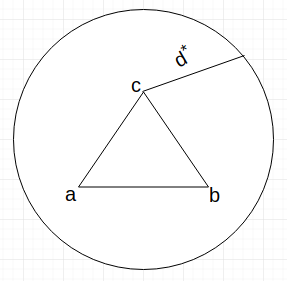
\includegraphics[width=10cm, height=7cm]{optimal_cluster.png}
\end{center}

where \textit{c} is the center of the optimal cluster, \textit{a} and \textit{b} are the centers from the clusters produced by the algorithm, and $ d^* $ is the cost. \\
We know that $ d(a,b) \leq 2d^* $ \\
From the triangle inequality we know that $ d(a,c) + (b,c) \geq d(a,b) $. \\
We also know that $ d(a,c) \leq d^*$ and $ d(b,c) \leq d^* $ \\
Then we get $ 2d^* \geq d(a+c) + d(b+c) \geq d(a,b) $ \\
From there we get that $ 2d^* \geq d(a,b) $, which can't happen because a and b are different centers which means that their distance should be $ \geq 2d^* $.

\newpage

\subsection{Prove that the STREAMING - FURTHEST algorithm is still a factor-2 approximation of the optimal clustering C on the data stream X }
From the algorithm we know that every point that is not a center has a distance to it's closest center smaller than two times the optimal distance. \\
In other words we can say that $ d \leq 2d^* $, where $ d $ is the distance from a point to it's nearest center and $ 2d^* $ is the maximum distance a point can have to it's closes cluster.
\\~\\
The first point that comes to the stream is a center because there are no other points.
\\~\\
When a value comes, it either becomes a new center or is assigned to a cluster. \\
If it's assigned to a cluster, we know that the distance from the point to it's closest cluster is smaller than two times the optimal distance.
$ d \leq 2d^* $.
\\~\\
The algorithm ends when then stream stops. \\
When the stream stops, all the values that are not centers are at distance $ d \leq 2d^* $ from their nearest centers. \\~\\

We can say that the cost of the clustering produced by the algorithm is some value $d_t$, which is $ d_t \leq 2d^* $. \\
With all the said, we can say that the algorithm is a factor-2 approximation of the optimal clustering C on the data stream X.


\subsection{Suggest how to modify the STREAMING - FURTHEST algorithm for the (realistic) case that the cost d ∗ of the optimal clustering is not known.}
 
\begin{lstlisting}
when the stream starts:
	read first k elements and assign them as centers
	d = (max distance between the centers) / 2

	read next element
	c = closest center
	conmpute the distance dm to its closest center
	if dm < d:
		assign it to that cluster
	else:
		# now we update the distance d
		d = dm + d
		remove c from the centers list
		assign the new element to be the center
\end{lstlisting} 

With this approach we basically read the first K elements and make them centers. Then we find the biggest distance between the k centers, divide it by 2 and that will be the \textit{cost}. \\
After the next element comes, we check it's distance to the closest center and if it is smaller, we assign it to that cluster. \\
If the distance is greater than the current cost, we update the cost to be the distance from the element to it's cluster + the previous distance. \\
Next we remove the closest center to the element from the centers list and assign the new element to be the center. \\
That way we always keep  \textit{k} number of centers. \\
This approach is not that optimal because the \textit{cost} can become large and the clusterss will have big radius and they will overlap a lot.

\section{Problem 3}
\subsection{Propose a streaming algorithm for deciding the connectivity of G(T, W )}

\begin{lstlisting}
vertex_array = []
edge_array = []

while edges are coming:
	# check is there is still space in the window
	if len(edge_array) == W:
		remove oldest edge from edge_array
	# add next edge to the edge_array
	edge_array.append(edge)
	# if node does not exist in the vertex_array, add it
	if node not in vertex_array:
		vertex_array.append(node)

	depth_first_search(W):
		find cycle
		remove oldest edge in the cycle

	# check connectivity
	if len(vertex_array) - len(edge_array) == 1:
		the graph is connected
	if len(vertex_array) - len(edge_array) > 1:
		the graph is disconnected
stop when the stream ends
\end{lstlisting}

Here is an explanation of the algorithm: \\
We keep track of the number of nodes and edges in the window. If $ num\_nodes - num\_edges = 1 $ then the graph is connected. If $ num\_nodes - num\_edges > 1 $, then the graph is disconnected. \\
We find a cycle in the graph using the depth first search traversal algorithm and remove the oldest edge in the cycle. \\
Whenever a new edge comes in the window, we remove the oldest edge in the graph G. We do that until the stream ends.

\subsection{Prove the correctness of your algorithm}
The algorithm tries to maintain a tree structure instead of a graph. That way we can always ensure that we have connectivity. \\
We achieve that by detecting a cycle as soon as it has been formed and we remove the oldest edge from it. That way we always have a tree unles an edge arrives that has vertices that have never been seen before, or an edge expires and we end up with an orphan node. In those cases the graph in disconnected. \\
Also the cycle can't be missed because depth first search algorithm always checks the whole tree. \\
Another thing to point out is that if we remove the oldest edge from the cycle, the three vertices will still be connected and when the time comes for that edge to be remove, we just shift the window. \\
Since we are always updating the number of edges and nodes, and we know that if $ node\_number - edge\_number = 1 $, then the graph is connected and if $ node\_number - edge\_number > 1 $, the the graph is disconnected. \\
That way we can always know the connectivity of the graph.

\subsection{How much space does your algorithm use?}
We are storing $ W $ edges and $ N $ nodes. \\
Depth-first search stores $ N $ visited nodes. \\
The space complexity in the worst case scenario is $ O(N^2W) $


\subsection{What is the update time of your algorithm?}
In worst scenarion the depth-first search algorithm needs to visit all the nodes in W, which takes $ O(N, W) $ time. \\
Checking if the elements that arrive are already present in the vertex array is instant so we don't include that in the calculation. \\
With that said, we can conclude that for the update process, we only need to consider the time for the depth-first search, which is $ O(N, W) $.


\end{document}



























